\documentclass[french]{beamer}

\usepackage[utf8]{inputenc}
\usepackage[T1]{fontenc}
\usepackage{lmodern}
\usepackage{amsmath, amssymb}
\usepackage{hyperref}

\usepackage{babel}


%CHOIX DU THEME et/ou DE SA COULEUR
% => essayer différents thèmes (en décommantant une des trois lignes suivantes)
\usetheme{PaloAlto}
%\usetheme{Madrid}
%\usetheme{Copenhagen}


% => il est possible, pour un thème donné, de modifier seulement la couleur
\usecolortheme{crane}
%\usecolortheme{seahorse}

%\useoutertheme[left]{sidebar}


%Pour le TITLEPAGE
\title{ \textbf{Développement d'un site web de contrôle de gestion sous Symfony 3}}
\subtitle{Stage fin d'étude\\ M2 Matis}
\author[]{ Sidi  MAOULOUD  \\ }
\date{Octobre 2017}
\institute[stage M2 Matis]{

\includegraphics[width=0.3\textwidth]{lh.png}
 
\includegraphics[width=0.3\textwidth]{logo.png} 
 \\

Université du Havre -- VMP-CONSULTING}


\begin{document}

\begin{frame}
	\titlepage
	

\end{frame}


\begin{frame}{Abstract}


	\begin{center}
\transblindshorizontal<1>[duration=1]	
	 \begin{block}

   
	VMP-Consulting is an office specialized in management control for small and medium-sized enterprises (SMEs), SMEs and local authorities. He accompanies them and advise them to move towards efficiency and efficiency in the use of their resources in order to achieve their objectives.
 \end{block}	
	\\
	
	\\
	
	\pause
	 \begin{block}
	 
	To better serve its customers, \textbf{VMP-CONSULTING}  wants to have a web portal for
implement a unique workspace for customers,
 offer customers privileged and personalized access to various services in
line, and
develop tools that enable clients to react with the contents of the
portal.\\
 \end{block}	
	\end{center}
	
	
\end{frame}






\begin{frame}{Plan}
\transsplitverticalin<1>[duration=1]

	\tableofcontents
\end{frame}

\section{Introduction}
\begin{frame}{Préambule}

\transglitter<1>[duration=1]



	\begin{exampleblock}{Contrôle de gestion}
	Un outil d’aide à la prise de décision qui évalue l’efficience et l’efficacité de la mise en œuvre des ressources de l’entreprise.
	\end{exampleblock}
	
\pause	
	
	\begin{exampleblock}{Utilité}
	C'est le garant de la bonne santé de l'entreprise en s'assurant que les ressources sont employées efficacement.
	\end{exampleblock}
	
\pause	
	
	\begin{exampleblock}{Pour le TPE/PME}
	  Il permet aux managers et aux opérationnels de se consacrer entièrement à leur cœur de métier,  et d'avoir une idée plus précise sur les coûts de l’entreprise, de mieux orienter la stratégie de l’entreprise et de leur procurer des outils de pilotage et de suivi des objectifs.

	 \end{exampleblock}
	
	
\end{frame}

\begin{frame}{VMP-CONSULTING}
\transblindshorizontal<1>[duration=1]	


\begin{block}{Objectifs}
\begin{itemize}

\item Maîtriser les coûts.

\item Optimiser les performances.

\item Une transparence sur la gestion des ressources de  l'entreprise.

\item Le développement de la réactivité dans la prise de décisions stratégiques.
\end{itemize}

\end{block}
\pause
\begin{block}{Services}
\begin{itemize}

\item \textbf{Pilotage d'entreprise } 


\item \textbf{Audi }


\item \textbf{Système d'information } 

\item \textbf{Formations }
\end{itemize}

\end{block}



	
\end{frame}


\begin{frame}{Problématique}
	\transblindshorizontal<1>[duration=1]	
    \begin{alertblock}{Un portail web}
    \begin{itemize}

 \item   Permettre la transmission des connaissances pour une organisation plus productive et performante
 \item     Améliorer le suivi des prestations réalisées par les consultants techniques 
 \item suivre en temps réel les interventions chez les clients
 
 \item   Renforcer  l'offre auprès des clients, les fidéliser avec de nouveaux services
 \item   Optimiser certaines tâches back-office 
\end{itemize}
   
	\end{alertblock} 
	\pause
	 \begin{alertblock}{Objectifs}
    \begin{itemize}

\item Améliorer la productivité des services de l'entreprise.
\item Fidéliser les clients.

\item Conquérir de nouveaux clients.
\end{itemize}
   
	\end{alertblock}   	
	
\end{frame}


\begin{frame}{Environnement et Missions}
	\transblindshorizontal<1>[duration=1]	
	\begin{block}{Environnement}
	VMP Consulting n'est pas une boite de développement.
	\end{block}
	\pause
	\begin{block}{Missions}
        	
	\begin{itemize}
\item Rédaction  du cahier des charges.
\item Analyse des données et proposition des solutions.
\item Conception  du site internet .  
\item Modélisation de la base de données.
\item Développement et Implémentation .
\item test et déploiement du portail web.
\end{itemize}
	
	\end{block}
	
	
\end{frame}


\section{Cahier des charges}
\begin{frame}{Cahier des charges}
	\transblindshorizontal<1>[duration=1]	
  \begin{block}{Le But}
  \begin{itemize}
\item \textbf{  Mettre en œuvre un espace de travail unique pour les clients}

\item \textbf{ Proposer aux clients un accès privilégié, personnalisé et sécurisé  à divers services en
ligne}
 
\item \textbf{ Développer des outils qui permettent aux clients de réagir avec les contenus du
portail}


\end{itemize}

\end{block}  	
	
	\begin{block}{Étude de l’existence }
	Les analyses et les calculs du futur système de gestion en ligne sont basés
sur des fichiers existants en Excel.
	\end{block}
	
\end{frame}


\begin{frame}{spécification fonctionnelle}

\transblindshorizontal<1>[duration=1]	
	\begin{exampleblock}{spécification fonctionnelle}
	\begin{itemize}
	
	\item L'accès au portail
	\item Création d’espace/entreprise
	\item Connexion
	\item Consultation des données
	\item Importation/Exportation
	\item Simulations
	
	\end{itemize}

	 \end{exampleblock}
	
	
	
	
	
\end{frame}

\begin{frame}{Cas d'utilisations}
\transblindshorizontal<1>[duration=1]	
\begin{center}


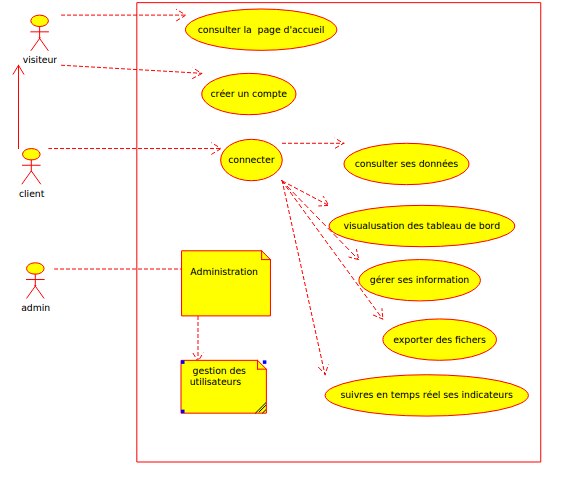
\includegraphics[width=0.9\textwidth]{cd2.png}
\end{center}

\end{frame}


\section{Conception}
\begin{frame}{Conception}
	\transblindshorizontal<1>[duration=1]	
\begin{center}
\begin{figure}[htp]
  \centering
  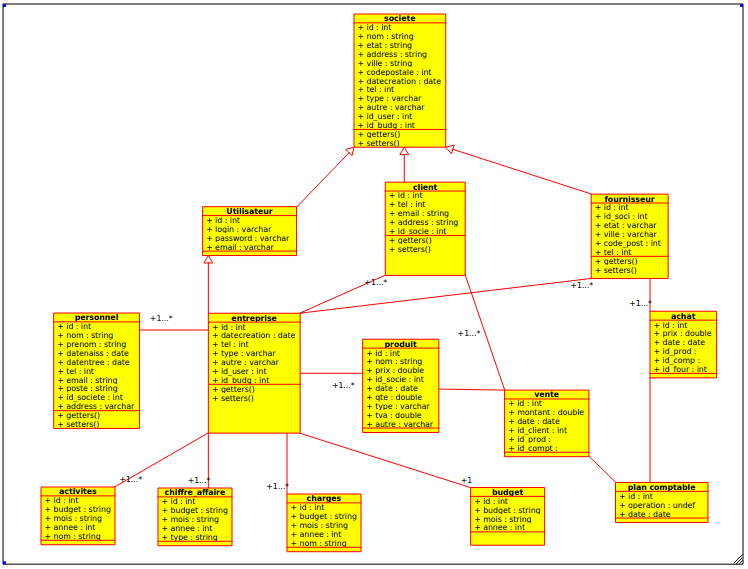
\includegraphics[width=8cm]{dc.png}
  \caption{Diagramme de classe.}
  \label{fig:une-autre-image}
\end{figure}

\end{center}	
	
	
\end{frame}

\begin{frame}{Le site web}
\transblindshorizontal<1>[duration=1]	
\begin{center}
\begin{figure}[htp]
  \centering
  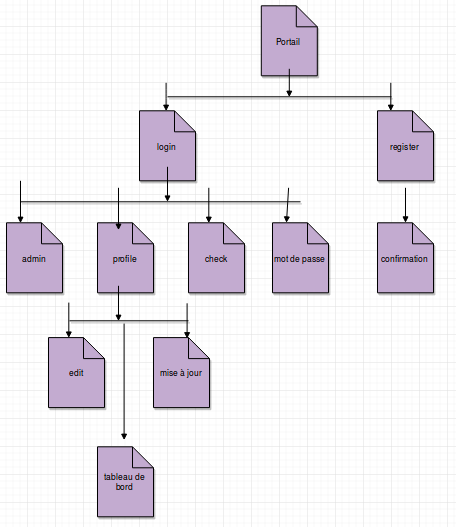
\includegraphics[width=6cm]{p3.png}
  \caption{Les templates principales du site  .}
  \label{fig:une-autre-image}
\end{figure}

\end{center}
\end{frame}


\begin{frame}{Modélisation}
\transblindshorizontal<1>[duration=1]	
	\begin{center}
\begin{figure}[htp]
  \centering
  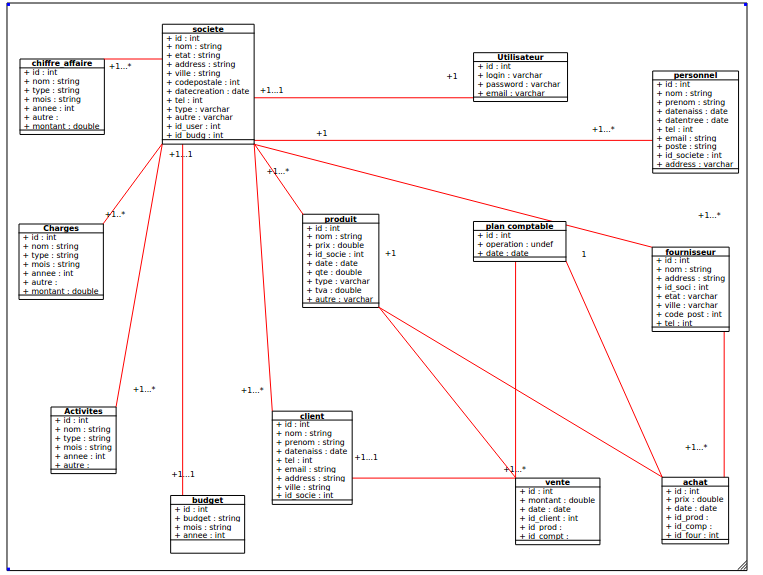
\includegraphics[width=8cm]{bd1.png}
  \caption{Les tables de la bases de données.}
  \label{fig:une-autre-image}
\end{figure}

\end{center}
\end{frame}

\begin{frame}{Maquette}
\transblindshorizontal<1>[duration=1]	
\begin{center}
\begin{figure}[htp]
  \centering
  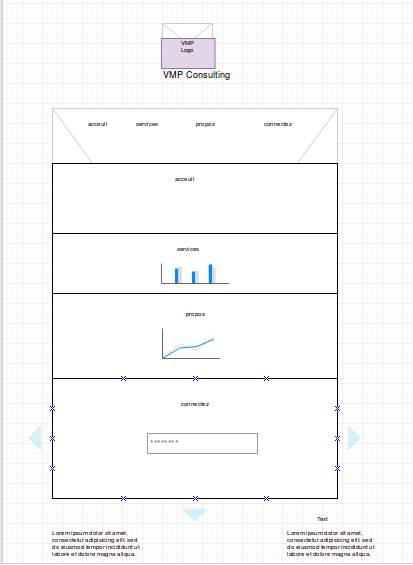
\includegraphics[width=6cm]{mod2.png}
  \caption{Maquette de la page d'accueil.}
  \label{fig:une-autre-image}
\end{figure}

\end{center}
\end{frame}

\section{Choix Techniques}
\begin{frame}{Coté serveur}
	\transblindshorizontal<1>[duration=1]	
\begin{exampleblock}{Méthodes}

\begin{itemize}
\item le codage  \textbf{from scratch}.
\item l'utilisation d'un \textbf{CMS}  .
\item \underline{l'utilisation d'un \textbf{framework} } .
\end{itemize}	

\end{exampleblock}
\pause

\begin{exampleblock}{Langages}

\begin{itemize}
\item \underline{ \textbf{PHP}}.
\item \textbf{JAVA (JEE)}  .
\item \textbf{JavaScript (NodeJS)} .
\end{itemize}	

\end{exampleblock}
\pause
\begin{exampleblock}{Framework}
	
\begin{itemize}
\item \underline{ \textbf{Symfony 3} }.
\item \textbf{Zend Framework 2}.
\item \textbf{Laravel}.
\end{itemize}

\end{exampleblock}
	
	
\end{frame}

\begin{frame}{Choix Techniques}
\transblindshorizontal<1>[duration=1]	

\begin{exampleblock}{Architecture}
	MVC permet d'organiser le code source.

\end{exampleblock}


\begin{exampleblock}{Base de données}

	\begin{itemize}
	\item Mysql (Modèle Relationnel)
	\item MongoDB (NoSql)
	\end{itemize}
	

\end{exampleblock}

\begin{exampleblock}{Coté client}
	\begin{itemize}
	\item HTML5
	\item CSS3 (Bootstrap)
	\item JavaScript (Jquery)
	\end{itemize}

\end{exampleblock}

\begin{exampleblock}{}
\begin{itemize}
\item git
\item Netbeans
\item phpmyadmin
  
\end{itemize}
\end{exampleblock}

\end{frame}



\section{Développement}
\begin{frame}{Front-End}
\transblindshorizontal<1>[duration=1]	
	\begin{block}{Twig}
	\begin{itemize}
	
\item	Un moteur de template moderne pour PHP, pour le développement des interfaces web.
	\item Il  a une syntaxe très concise, qui rend les modèles plus lisibles.
	\item L'un des objectifs de \textbf{Twig} est d'être le plus rapide possible.
	\item L'Héritage.
		\end{itemize}

	\end{block}
	\pause
\begin{block}{Espace client}
	\textbf{FOSUserBundle} est un bundle qui s'occupe de gestion des utilisateurs.
	\end{block}
	\pause
	\begin{block}{Tableau de bord}
	\textbf{CMENGoogleChartsBundle} permet de faire des Dashboard.
	\end{block}	
	
\end{frame}


\begin{frame}{Les Entités}
\transblindshorizontal<1>[duration=1]	
\begin{block}{Doctrine}
se charge de l'enregistrement des  données en  faisant oublier qu'il y a une base de données.\\
Pour enregistrer les entités on utilise le service \textbf{EntityManager}.\\
Et pour la récupération des données, on utilise les repositories
\end{block}
\pause
\begin{block}{Les relations}
Les notions de propriétaire et d'inverse, et de  unidirectionnalité et de bidirectionnalité sont  importantes dans les relation Doctrine.
\begin{itemize}
\item OneTone
\item OneToMany
\item ManyToMany

\end{itemize}
\end{block}

\end{frame}

\begin{frame}{Administration et Sécurité}
\transblindshorizontal<1>[duration=1]	
\begin{alertblock}{Back-Office}
le bundle \textbf{EasyadminBundle}  est facile à configurer.
\end{alertblock}	


\begin{alertblock}{Sécurité}
\begin{itemize}
\item \textbf{authentification} 
\item \textbf{autorisation}
\end{itemize}

Processus:
\begin{enumerate}
\item    Un utilisateur veut accéder à une ressource protégée 

 \item    Le firewall redirige l'utilisateur au formulaire de connexion 

  \item   L'utilisateur soumet ses informations d'identification 

 \item    Le firewall authentifie l'utilisateur 

 \item    L'utilisateur authentifié renvoie la requête initiale 

 \item    Le contrôle d'accès vérifie les droits de l'utilisateur, et autorise ou non l'accès à la ressource protégée.
\end{enumerate}

\end{alertblock}	
	
	
\end{frame}

\begin{frame}{Sécurité}
\transblindshorizontal<1>[duration=1]	
\begin{center}
\begin{figure}[htp]
  \centering
  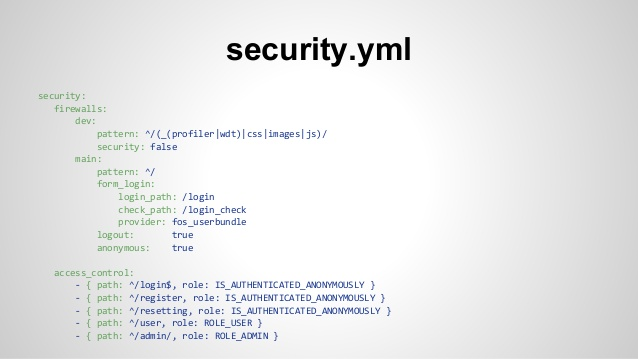
\includegraphics[width=12cm]{s.jpg}
  \caption{security.yml.}
  \label{fig:une-autre-image}
\end{figure}

\end{center}

\end{frame}

\begin{frame}{Temps réel}
\transblindshorizontal<1>[duration=1]	
\begin{alertblock}{Ajax}
\begin{itemize}
\item un script qui fait appel à une page php toutes les 5 secondes
\item Un système \textbf{push AJAX}
\end{itemize}
\end{alertblock}	
\pause
\begin{alertblock}{WebSocket}
\begin{itemize}
\item utiliser  un adaptateur \textbf{SocketIO} pour PHP, un serveur  \textbf{NodeJS}.
\item utiliser \textbf{Ratchet}
\end{itemize}
\end{alertblock}
	
	
\end{frame}

\section{Tests}
\begin{frame}{Tests}
\transblindshorizontal<1>[duration=1]	
\begin{center}

\href{http://localhost:8000/Portail}{
\includegraphics[width=0.8\textwidth]{v1.png} }

	
	
	
\end{center}
\end{frame}


\section{Conclusion}
\begin{frame}{Conclusion}
\transblindshorizontal<1>[duration=1]	
	\begin{exampleblock}{}
	\begin{itemize}
	\item Ce stage au sein de l'entreprise VMP-CONSULTING termine ses premiers 4 mois , mais en réalité le vrai développement ne fait que commencer.
	\item La rédaction du cahier des charges seule était une expérience importante dans ma vie professionnelle.
	\item Ce stage est une opportunité pour la réalisation d'un site web de A à Z, il m'a permis d’être le concepteur, le designer, et le développeur d'un projet informatique, mais aussi il est un défi de réaliser toutes ces missions seul.
	\item il était une occasion d'explorer le responsive design avec \textbf{Bootstrap}, le JavaScript avec Jquery, et le temps réel avec le WebSocket.\\
En plus Ce site web est  mon premier projet professionnel développé sous \textbf{Symfony}.
	\end{itemize}
	\end{exampleblock}
\end{frame}


\section{Bibliographie}
\begin{frame}{Bibliographie}
	


\begin{thebibliography}{10}
    
  \beamertemplatebookbibitems
  % Start with overview books.

  \bibitem{www.openclassrooms.com}
   www.openclassrooms.com.
    \newblock {\em cours Symfony}.
    \newblock .
 
     \bibitem{www.symfony.com}
   www.symfony.com.
    \newblock {\em Symfony}.
    \newblock Documentation.
    
      \bibitem{www.symfony.com}
    www.symfony.com.
    \newblock {\em Twig}.
    \newblock Documentation.
    
      \bibitem{www.doctrine-project.org}
   www.doctrine-project.org.
    \newblock {\em Doctrine}.
    \newblock Documentation.

\bibitem{getbootstrap.com}
 getbootstrap.com
    \newblock {\em Bootstrap}.
    \newblock Documentation.
    
   
    
    
      \bibitem{www.symfony.com}
    www.symfony.com.
    \newblock {\em EasyAdminBundle}.
    \newblock Documentation.
   
    
     
   
  \end{thebibliography}
\end{frame}

\begin{frame}{Questions}
\begin{center}
{\LARGE Je vous remercie pour votre attention.}\\
\\
\\

\\
{\Large Questions ?}
\end{center}
\end{frame}

\end{document}
